\documentclass[10pt,letterpaper]{article}
\usepackage[top=0.85in,left=2.75in,footskip=0.75in]{geometry}

% amsmath and amssymb packages, useful for mathematical formulas and symbols
\usepackage{amsmath,amssymb}

\usepackage{soul}
%\sethlcolor{white}

% Use adjustwidth environment to exceed column width (see example table in text)
\usepackage{changepage}

% Use Unicode characters when possible
\usepackage[utf8x]{inputenc}

% textcomp package and marvosym package for additional characters
\usepackage{textcomp,marvosym}

% cite package, to clean up citations in the main text. Do not remove.
%\usepackage{cite}

\usepackage[sort&compress,numbers]{natbib}
%\bibliographystyle{unsrtnat}
\bibliographystyle{plos2015}

% Use nameref to cite supporting information files (see Supporting Information section for more info)
\usepackage{nameref,hyperref}

\hypersetup{
    colorlinks,
    linkcolor={red!50!black},
    citecolor={blue!50!black},
    urlcolor={blue!80!black}
}

% line numbers
\usepackage[right]{lineno}

% ligatures disabled
\usepackage{microtype}
\DisableLigatures[f]{encoding = *, family = * }

% color can be used to apply background shading to table cells only
\usepackage[table]{xcolor}

% array package and thick rules for tables
\usepackage{array}

% create "+" rule type for thick vertical lines
\newcolumntype{+}{!{\vrule width 2pt}}

% create \thickcline for thick horizontal lines of variable length
\newlength\savedwidth
\newcommand\thickcline[1]{%
  \noalign{\global\savedwidth\arrayrulewidth\global\arrayrulewidth 2pt}%
  \cline{#1}%
  \noalign{\vskip\arrayrulewidth}%
  \noalign{\global\arrayrulewidth\savedwidth}%
}

% \thickhline command for thick horizontal lines that span the table
\newcommand\thickhline{\noalign{\global\savedwidth\arrayrulewidth\global\arrayrulewidth 2pt}%
\hline
\noalign{\global\arrayrulewidth\savedwidth}}


% Remove comment for double spacing

%\usepackage{setspace}
%\doublespacing

% Text layout
\raggedright
\setlength{\parindent}{0.5cm}
\textwidth 5.25in 
\textheight 8.75in

% Bold the 'Figure #' in the caption and separate it from the title/caption with a period
% Captions will be left justified
\usepackage[aboveskip=1pt,labelfont=bf,labelsep=period,justification=raggedright,singlelinecheck=off]{caption}
\renewcommand{\figurename}{Fig}

% Remove brackets from numbering in List of References
\makeatletter
\renewcommand{\@biblabel}[1]{\quad#1.}
\makeatother

% Header and Footer with logo
\usepackage{lastpage,fancyhdr,graphicx}
\usepackage{epstopdf}
%\pagestyle{myheadings}
\pagestyle{fancy}
\fancyhf{}
%\setlength{\headheight}{27.023pt}
%\lhead{\includegraphics[width=2.0in]{PLOS-submission.eps}}
\rfoot{\thepage/\pageref{LastPage}}
\renewcommand{\headrulewidth}{0pt}
\renewcommand{\footrule}{\hrule height 2pt \vspace{2mm}}
\fancyheadoffset[L]{2.25in}
\fancyfootoffset[L]{2.25in}
\lfoot{\today}

%% END MACROS SECTION

\widowpenalty10000
\clubpenalty10000

\begin{document}
\vspace*{0.2in}

% Title must be 250 characters or less.
\begin{flushleft}
{\Large
\textbf\newline{Tximeta: reference sequence checksums for provenance identification in RNA-seq}
}
\newline
\\
Michael I. Love\textsuperscript{1,2*},
Charlotte Soneson\textsuperscript{3,4},
Peter F. Hickey\textsuperscript{5,6},
Lisa K. Johnson\textsuperscript{7},
N. Tessa Pierce\textsuperscript{7},
Lori Shepherd\textsuperscript{8},
Martin Morgan\textsuperscript{8},
Rob Patro\textsuperscript{9}
\\
\bigskip
\textbf{1} Department of Biostatistics, University of North Carolina-Chapel Hill, Chapel Hill, NC, USA
\\
\textbf{2} Department of Genetics, University of North Carolina-Chapel Hill, Chapel Hill, NC, USA
\\
\textbf{3} Friedrich Miescher Institute for Biomedical Research, Basel, Switzerland
\\
\textbf{4} SIB Swiss Institute of Bioinformatics, Basel, Switzerland
\\
\textbf{5} Epigenetics and Development Division, The Walter and Eliza Hall Institute of Medical Research, 1G Royal Parade, Parkville VIC 3052, Australia
\\
\textbf{6} The Department of Medical Biology, University of Melbourne, Parkville VIC 3010, Australia
\\
\textbf{7} Department of Population Health and Reproduction, University of California, Davis, Davis, California, USA
\\
\textbf{8} Roswell Park Comprehensive Cancer Center, Buffalo, NY, USA
\\
\textbf{9} Department of Computer Science, University of Maryland, College Park, MD, USA
\\
\bigskip

% Use the asterisk to denote corresponding authorship and provide email address in note below.
* michaelisaiahlove@gmail.com

\end{flushleft}

% Please keep the abstract below 300 words
\section*{Abstract}

Correct annotation metadata is critical for reproducible and accurate
RNA-seq analysis. When files are shared publicly or among
collaborators with incorrect or missing annotation metadata, it
becomes difficult or impossible to reproduce bioinformatic analyses
from raw data. It also makes it more difficult to locate the
transcriptomic features, such as transcripts or genes, in their proper
genomic context, which is necessary for overlapping expression data
with other datasets. We provide a solution in the form of an
R/Bioconductor package tximeta that performs numerous annotation and
metadata gathering tasks automatically on behalf of users during the
import of transcript quantification files. The correct reference
transcriptome is identified via a hashed checksum stored in the
quantification output, and key transcript databases are downloaded and
cached locally. The computational paradigm of automatically adding
annotation metadata based on reference sequence checksums can greatly
facilitate genomic workflows, by helping to reduce overhead during
bioinformatic analyses, preventing costly bioinformatic mistakes, and
promoting computational reproducibility.
The tximeta package is
available at \url{https://bioconductor.org/packages/tximeta}.

\linenumbers

\section*{Introduction}

An RNA-seq data analysis often involves quantification of sequence
read data with respect to a set of known reference transcripts. These
reference transcripts may be downloaded from a database such as
GENCODE, Ensembl, or RefSeq \cite{gencode,ensembl,refseq} in the form
of nucleotide sequences in FASTA format and/or transcript locations in a genome in
GTF/GFF (gene transfer format / general feature format). Alternatively
a novel set of reference transcripts may be derived as part of the data analysis. The
provenance of the reference transcripts, including their source and release
number, can be considered critical metadata with respect to the
processed data, that is, the files with quantification information. Without
information about the reference provenance, computational
reproducibility --- re-performing the analysis with the same data and
code and obtaining the same result~\cite{Patil2016} --- 
may be difficult or impossible. Reproducibility has been set as a
high-level goal for all NIH-funded research~\cite{collins2014,lauer2017}, 
and so as developers of bioinformatic tools, we should design software
that promotes and facilitates computational reproducibility.
Manually keeping track of
critical pieces of metadata throughout a long-term bioinformatic
project is tedious and error prone; still, manual metadata tracking is
a common practice in RNA-seq bioinformatics. For example, a common
approach to tracking the reference transcripts that were used during
quantification would be to keep a \texttt{README} file in the same
directory as the quantification data, with information about the
provenance of the reference transcripts.

In addition to impeding computational reproducibility, missing or
wrong metadata can potentially lead to serious errors in downstream
analysis: if quantification data are shared with genomic coordinates
but without critical metadata about the genome version, computation of
overlaps with other genomic data with mis-matching genome versions can
lead to faulty inference of overlap enrichment. Additional annotation
tasks, such as conversion of transcript or gene identifiers, or
summarization of transcript-level data to the gene level is made more difficult
when the reference provenance is not known. Kanduri \textit{et al.}~\cite{Kanduri2017}
documented issues surrounding the lack of provenance metadata for BED,
WIG, and GFF files, and described this problem as a ``major time
thief'' in bioinformatics. Likewise, Simoneau and
Scott~\cite{Simoneau2019} described 
information on genome assembly and annotation as ``essential'' for
describing the computational analysis of RNA-seq data, and contended
that, ``no study using RNA-seq should be published without these
methodological details.'' \hl{Simoneau and co-authors have recently
performed a detailed analysis of hundreds of published RNA-seq studies
finding that the majority did not include annotation source and release
information, thus hindering reproducible analysis}~\cite{Simoneau2019BIB}.

A number of frameworks have been proposed that would solve the problem
of tracking provenance in a bioinformatic analysis -- provenance in
the narrow sense defined above, encompassing the source and release
information of the reference sequence -- as well as in a larger sense
of tracking the state of all files, including data and metadata and
any software used to process these files, throughout every step of an
analysis. We will first review frameworks for tracking provenance of
reference sequences, and secondly describe more general
frameworks. The CRAM format, developed at the European Bioinformatics
Institute, involves computing differences between biological sequences
and a given reference so that the sequences themselves do not need to
be stored in full within an alignment file \cite{cram}. Because the
specific reference used for compression is critical for data
integrity, CRAM includes checksums of the reference sequences as part
of the file header. A partner utility called refget has been developed
in order to allow for programmatic retrieval of the reference sequence
from a computed checksum, which acts as an identifier of the reference
sequence \cite{refget}. A similar approach is taken by the Global
Alliance for Genomics and Health's (GA4GH) Variation Representation
Specification (VR-Spec) \cite{vr}, which uses a hashed checksum (or
``digest'') to uniquely refer to molecular variation, and by the
seqrepo python package for writing and reading collections of
biological sequences \cite{seqrepo}. The NCBI Assembly database takes
a different approach, by assigning unambiguous identifier strings
(though not computed via a hash function) to sets of sequences
comprising specific releases of a genome assembly
\cite{ncbi-assembly}. Knowing the identifier is therefore sufficient
to know the full set of sequences in the assembly.
Another approach to reduce manual metadata tracking associated with a
number of reference sequences is Refgenie. Refgenie is a tool that
helps with management of bundles of files associated with reference
genomes, and facilitates sharing provenance information across
research groups, in that the generation of resources is scripted
\cite{refgenie}.
\hl{TODO fix this} Arkas, ARMOR, pepkit, and basejump are all
frameworks for automating bioinformatic analyses, where reference
provenance is specified in configuration files and correct metadata
can therefore be assembled and attached programmatically to downstream
outputs \cite{arkas,Orjuelag2019,pepkit,basejump}.

In 2015, Belhajjame \textit{et al.}~\cite{Belhajjame2015} introduced
the concept of a ``Research Object'', an aggregation of data and
supporting metadata produced within a specified scientific
workflow. Their formulation was system-neutral, describing the
requirements for production of a Research Object. The requirements
touch on topics introduced above, such as the need to preserve data
inputs, software versions, as well as traces of the provenance of data
as it moves through the scientific workflow. Belhajjame
\textit{et al.}~\cite{Belhajjame2015} summarized literature in the field of
computational reproducibility and efforts toward extensive provenance
tracking. The developers of the Common Workflow Language (CWL)
\cite{cwl} have defined a profile, CWLProv, for recording provenance
through a workflow run, and have a number of implementations,
including within cwltool \cite{Khan2018}. The developers of CWLProv
emphasized the importance of tracking versions of input data, such as
reference genomes or variant databases in a scientific workflow, and
they suggested to use and store stable identifiers of all data and
software, as well as the workflow itself. As identifiers play such a
crucial role in assuring reproducibility of workflows, the developers
of CWLProv recommended the use of hashed checksums for identifiers of
data (including any reference sequence), similar to the use of
checksums in the CRAM format and VR-Spec, for identifying the
reference or variant sequences. Gruning
\textit{et al.}~\cite{Gruning2018} recommended combining systems such as Galaxy
for encapsulating analysis tools with systems for tracking and
capturing parameters and source data provenance to provide full
computational reproducibility.

Here we describe an R/Bioconductor package, tximeta, for
identification of reference transcript provenance in RNA-seq analyses
via sequence checksums. It is situated among other solutions for
facilitating computational reproducibility described above, with some
automation of routine tasks, such as conversion of transcript and gene
names, but short of full automation of \hl{downstream statistical} analyses
as in Arkas and ARMOR. Tximeta captures the versions of the software
packages used in import of quantification data, but does not provide
full provenance tracking throughout downstream tasks as in the
Research Object specification or in CWLProv. One \hl{unique} aspect of
tximeta is that -- through the use of hashed checksums of reference
transcripts and lookup operations similar to those performed by refget
-- our implementation can be used to identify the reference provenance
\textit{post hoc} on various shared or public datasets, regardless of
whether the original analyst kept or shared accurate records of the
reference transcripts that were used. Therefore it can provide some
utility for bioinformatic analysts without requiring full buy-in of a
particular workflow execution framework.
\hl{\textit{Post hoc} transcriptome identification is a novel
functionality not offered by alternative exiting pipelines for
importing or creating RNA-seq count matrices in R/Bioconductor.}
Tximeta is similar in implementation to the CRAM format in the use of
hashed checksums, but identifies the transcript sequences used during
\hl{RNA-seq} sample quantification rather than the genome sequence
used during alignment. We see tximeta as a piece of a larger effort to
create software systems that are ``more amenable to reproducibility''
\cite{Peng2011}.

\section*{Design and Implementation}

Tximeta has been developed to work with output from Salmon
or alevin quantification tools \cite{salmon,alevin},
although the implementation could be extended to other quantification
tools that store the appropriate hashed checksum within the index and propagate this
checksum to the sample output metadata. Without loss of generality, we
describe the implementation referring to Salmon quantification data
below. A diagram of the following workflow is shown in Figure
\ref{fig:diagram}. 

\begin{figure}
  \centering
  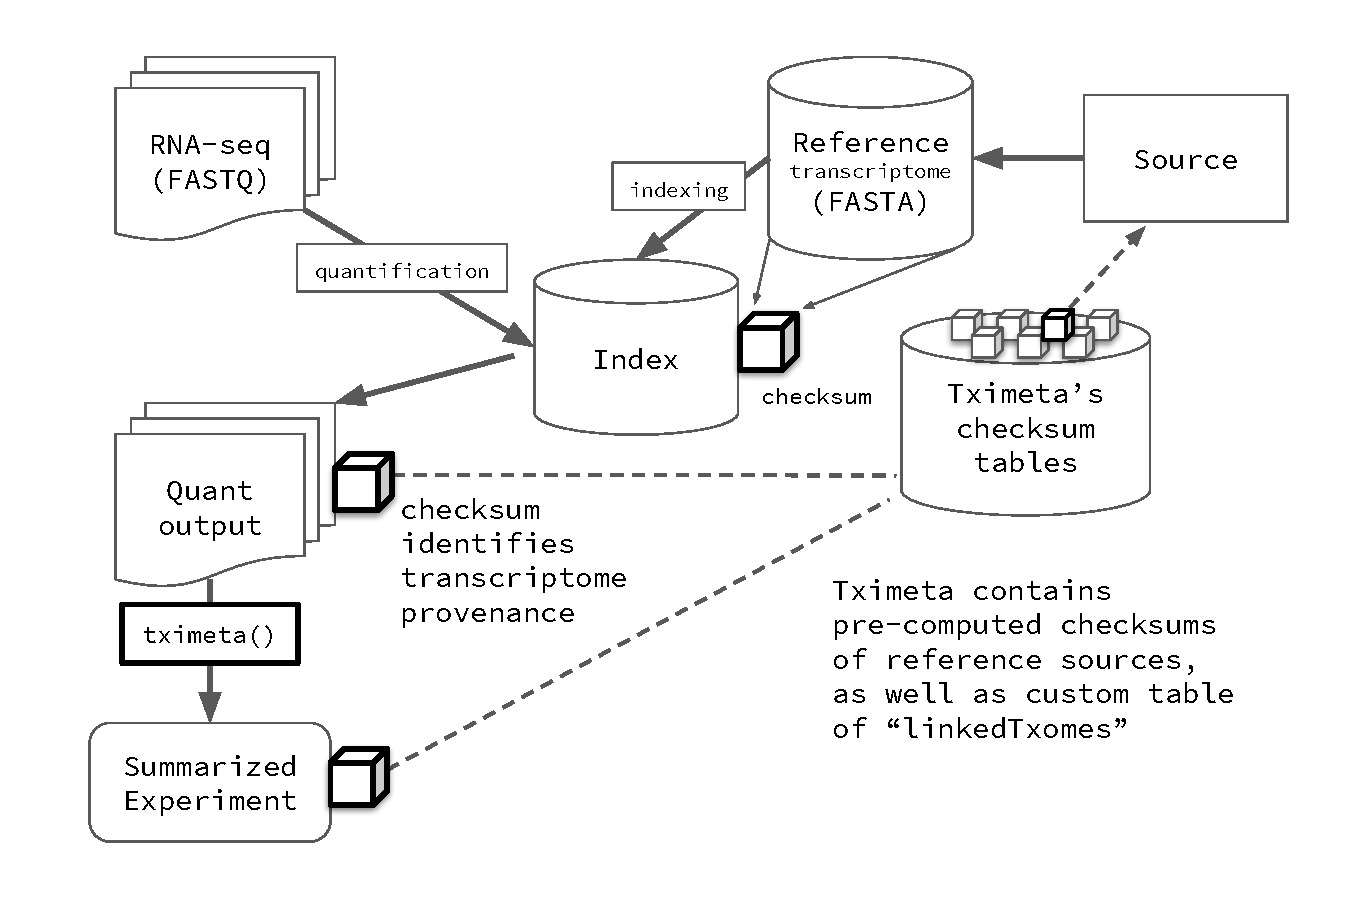
\includegraphics[width=\textwidth]{diagram.pdf}
  \caption{
    {\bf Flowchart of Salmon quantification followed by tximeta.}
    The quantification and import pipeline results in a
    SummarizedExperiment object with reference transcript provenance
    metadata added by tximeta (see Design and Implementation).
    \hl{The SummarizedExperiment object contains estimated counts and
    other relevant metadata, and can be used with downstream
    statistical packages.}}
  \label{fig:diagram}
\end{figure}

During the indexing step, Salmon computes the hashed checksum of the
cDNA sequence of the reference transcripts. The set of reference
transcripts provided to Salmon will be referred to in this text as the
\textit{transcriptome}, although we note that the reference is not
necessarily equal to the complete set of possible RNA transcripts in
the sample. Currently, both the SHA-256 and SHA-512 \cite{sha1}
checksums are computed on the reference cDNA sequences alone, with
transcript sequences concatenated together with the empty string (the
SHA-256 checksum is currently taken as the primary identifier). Future
implementations of Salmon and tximeta may use alternate hash functions
for compatibility with larger efforts toward stable identifiers for
sequence collections, for example, computing a hashed checksum over a
lexicographically sorted set of checksums for each transcript cDNA
sequence, which would provide order-invariance for the collection
identifier. During quantification of a single sample, Salmon embeds
the transcriptome index checksum in a metadata file associated with
the sample output. For each sample, Salmon outputs a directory with a
specific file structure, including files with quantification
information as well as others with important metadata about the
parameters. The entire directory, not just the text file with the
quantification information, should be considered the output of
the quantification tool.

During import of quantification data into R/Bioconductor
\cite{bioc}, leveraging the existing tximport package
\cite{tximport}, tximeta reads the quantification data, as well as
the transcriptome index checksum, and compares this checksum to a hash
table of pre-computed checksums of a subset of commonly used reference
transcriptomes (human, mouse, and fruit fly reference transcripts from
GENCODE, Ensembl, and RefSeq, see Table \ref{tab:hash}), as well as to a
custom hash table which will be described below. Tximeta verifies that
the checksum and therefore the reference transcriptome sequence is
identical across all samples being imported. If there is a match of
the checksum among the pre-computed checksums or in the custom hash table,
tximeta will begin to compile additional relevant
metadata. Depending on whether the checksum has been seen by tximeta
before, one of two steps will occur:

\begin{itemize}
\item (First time) - Tximeta attempts to download the appropriate GTF/GFF
  file via FTP and parse it using Bioconductor packages. 
  GENCODE and RefSeq GTF/GFF files are parsed
  by GenomicFeatures \cite{granges}, while Ensembl GTF files are
  parsed by ensembldb \cite{ensembldb}. Tximeta then creates a
  locally cached SQLite database of the parsed GTF/GFF file, as well as a
  GRanges object of the transcript locations \cite{granges}. The
  local cache is managed by the BiocFileCache Bioconductor package
  \cite{biocfilecache}. \hl{If the database for the correct Ensembl
    release is available using Bioconductor's AnnotationHub
    infrastructure, this pre-parsed database will be downloaded
    instead of downloading and parsing the GTF.}
\item (Subsequently) - Tximeta loads the locally cached versions of
  metadata (the transcript ranges, or additionally the SQLite database
  on demand for further annotation tasks).
\end{itemize}

After loading the appropriate annotation metadata, tximeta outputs a
SummarizedExperiment object \cite{granges}, a class in the
Bioconductor ecosystem which stores multiple similarly shaped matrices
of data, or ``assays'', including the estimated read counts, effective
transcript lengths, and estimates of abundance (in transcripts per
million, TPM). By convention, rows correspond to genomic features
(e.g. transcripts or genes), while columns correspond to samples. In
addition, the rows of the matrices are linked to transcript ranges,
embedded in an appropriate genome version (e.g. GRCh38) including
chromosome names and lengths. \hl{The SummarizedExperiment object can
then be used with downstream statistical analysis packages in
Bioconductor, as described in the tximeta software vignette.}

If tximeta did not find a matching
transcriptome in the hash table then a non-ranged SummarizedExperiment
will be returned as the function's output, as the location and context
of the transcript ranges are not known to tximeta. Comparison of
ranges across genome versions, or without properly matching
chromosomes, will produce an error, leveraging default functionality
from the underlying GenomicRanges package \cite{granges}. Metadata
about the samples, if provided by the user, is automatically attached
to the columns of the SummarizedExperiment object. Additional metadata
attached by tximeta includes all of the per-sample metadata saved from
Salmon (e.g. library type, percent reads mapping, etc.), information
about the reference transcriptome and file paths or FTP URLs for the source file(s)
for FASTA and GTF/GFF, and the package versions for tximeta and other
Bioconductor packages used during the parsing of the GTF/GFF. At any
later point in time, annotation tasks can be performed by on-demand
retrieval of the cached databases, for example summarization of
transcript-level information to the gene level, conversion of
transcript or gene identifiers, or addition of exon ranges.

A key aspect of the tximeta workflow described here is that it does
not rely on self-reporting of the reference provenance for
\textit{post hoc} identification of the correct metadata. An exception
to this rule is the case of a \textit{de novo} constructed
transcriptome, or in general, use of a transcriptome that is not yet
contained in tximeta's built-in hash table of reference
transcriptomes. For such cases, we have developed functionality in
tximeta to formally link a given hashed checksum to a publicly
available FASTA file(s) and a GTF/GFF file. The
\texttt{makeLinkedTxome} function can be called, pointing to the
transcriptome index as well as to the locations of the FASTA files and
GTF/GFF file, and this will perform two operations:
(1) it will add a row to a custom hash
table, managed by BiocFileCache, and (2) it will produce a JSON file
that can be shared or uploaded to public repositories,
which links the transcriptome checksum
with the source locations. When the JSON file is provided to
\texttt{loadLinkedTxome} on another machine, it will add the relevant
row to tximeta's custom hash table, so tximeta will then recognize and
automatically populate metadata in a similar manner to if the checksum
matched with a transcriptome in tximeta's built-in hash
table. Finally, the cache location for tximeta, managed by
BiocFileCache, can be shared across users on a cluster, for example,
such that parsed databases, range objects, and custom hash tables
created by any one user can be leveraged by all other users in the
same group.

\begin{table}[t]
  \centering
  \caption{\bf{Comparison of tximeta to related software.}}
\begin{tabular}{llccc} 
  \hline
  \bf{Software} & \bf{Domain} & \bf{Ranges} & \bf{Release} & \bf{Post hoc} \\
   & & \bf{autom.}   & \bf{autom.}   & \bf{lookup}   \\
   & & \bf{attached} & \bf{attached} & \bf{possible} \\
  \thickhline
  \underline{tximeta} & RNA-seq import                  & \checkmark & \checkmark & \checkmark \\
  tximport \cite{tximport} & RNA-seq import             & & & \\
  \hline
  Arkas \cite{arkas} & RNA-seq analysis                 & & & \\
  ARMOR* \cite{Orjuelag2019} & RNA-seq analysis         & \checkmark & \checkmark & \checkmark \\
  \hline
  htseq \cite{htseq} & RNA-seq counting                 & & & \\
  featureCounts \cite{featurecounts} & RNA-seq counting & \checkmark & & \\
  summarizeOverlaps \cite{granges} & RNA-seq counting   & \checkmark & \checkmark & \\
  \hline
  pepkit \cite{pepkit} & Workflow mngmt.                & - & - & \\
  basejump \cite{basejump} & Metadata utilities         & - & - & \\
  Refgenie \cite{refgenie} & Genome mngmt.              & - & - & \checkmark \\
  CRAM+RefGet \cite{cram,refget} & Read alignment       & - & - & \checkmark \\
  CWLProv \cite{Khan2018} & Workflow tracing            & - & - & \checkmark \\
\hline
\end{tabular}
\begin{flushleft}
  \hl{Tximeta is compared to related software, grouped by domain.
    Columns indicate if the transcript or gene ranges are automatically
    attached the output of the software, whether the transcriptome and
    genome release information is automatically attached, and whether
    \textit{post hoc} lookup of transcriptome-related metadata is possible.
    A hyphen (-) indicates that the column is not directly applicable.
    *Note that ARMOR imports tximeta for building SummarizedExperiment
    objects.}
\end{flushleft}
\label{tab:comp}
\end{table}

\subsection*{Comparison to related software}

\hl{A number of related software projects are compared with respect to
  key features of tximeta in} Table~\ref{tab:comp}. \hl{While other
  RNA-seq pipelines exist to import quantification data into
  R/Bioconductor, tximeta uniquely allows for \textit{post hoc}
  identification of the reference sequence provenance.  The most
  directly related RNA-seq packages create a SummarizedExperiment, or
  an object of similar shape and function, including}
Arkas \cite{arkas}, ARMOR \cite{Orjuelag2019},
htseq \cite{htseq}, featureCounts \cite{featurecounts} from the
Rsubread package, and summarizeOverlaps \cite{granges} from the
GenomicAlignments package. 
\hl{Arkas imports transcript-level quantification data, but does not
  attach transcript ranges or release information. ARMOR depends on
  tximeta, and so relies on functionality described here to attach
  transcript ranges and release information to the output object.}

\hl{The software htseq, featureCounts, and summarizeOverlaps all
  perform counting operations for aligned RNA-seq reads with
  respect to specific gene models, and can be used to generate an
  R/Bioconductor object similar to that provided by tximeta.  The
  htseq python package and subsequent data import with DESeq2 create a
  SummarizedExperiment, but without ranges or release information
  attached. The R functions featureCounts and summarizeOverlaps
  automatically attach ranges, and the latter will also attach the
  transcriptome release metadata, given that a GenomicRanges object
  was used to perform the counting operation. However, neither
  featureCounts nor summarizeOverlaps allow for \textit{post hoc}
  metadata operations, such as the addition or modification of ranges,
  or addition of relevant metadata, as they do not explicitly connect
  the object with a remote or locally cached database as tximeta
  does.}

\hl{Other software such as}
pepkit \cite{pepkit}, basejump \cite{basejump},
Refgenie \cite{refgenie},
CRAM \cite{cram}, refget \cite{refget}, and
CWLProv \cite{Khan2018}
\hl{are not particularly designed for RNA-seq data import, and so are
  less directly comparable to tximeta. Pepkit, basejump, Refgenie, and
  CWLProv are generic workflow or resource management tools, some of
  which allow for the possibility of \textit{post hoc} identification
  of annotation metadata. However, none of these would provide
  automatic metadata attachment (range and release information) for
  RNA-seq as accomplished by tximeta.}

\begin{table}[t]
  \centering
  \caption{\bf{Pre-computed reference transcripts checksums as of Fall 2019.}}
\begin{tabular}{llll} 
  \hline
  \bf{Source} & \bf{Organism} & \bf{Releases} & \bf{Transcript sequence file} \\
  \thickhline
  GENCODE & \textit{Homo sapiens} & 23 -- 32 & transcripts.fa \\
  GENCODE & \textit{Mus musculus} & M6 -- M23 & transcripts.fa \\
  \hline
  Ensembl & \textit{Homo sapiens} & 76 -- 98 & *.cdna.all.fa (NR) \\
  Ensembl & \textit{Mus musculus} & 76 -- 98 & *.cdna.all.fa (NR) \\
  Ensembl & \textit{Drosophila melanogaster} & 79 -- 98 & *.cdna.all.fa (NR) \\
  \hline
  Ensembl & \textit{Homo sapiens} & 76 -- 98 & *.cdna.all.fa + *.ncrna.fa \\
  Ensembl & \textit{Mus musculus} & 76 -- 98 & *.cdna.all.fa + *.ncrna.fa \\
  Ensembl & \textit{Drosophila melanogaster} & 79 -- 98 & *.cdna.all.fa + *.ncrna.fa \\
  \hline
  RefSeq & \textit{Homo sapiens} & p1 -- p12$\dagger$ & *\_rna.fa \\
  RefSeq & \textit{Mus musculus} & p2 -- p5$\dagger$ & *\_rna.fa \\
\hline
\end{tabular}
\begin{flushleft}
  The set of pre-computed checksums span the stable releases from
  these sources for the years 2015 -- 2019. (NR) - not recommended: we
  recommend combination of coding and non-coding transcripts for
  accurate RNA-seq quantification; $\dagger$ - RefSeq assembly
  versions p13 and p6 for human and mouse respectively are currently
  ``latest'', and are subject to sequence updates under the same
  assembly version, and so not stable releases.
\end{flushleft}
\label{tab:hash}
\end{table}

\section*{Results}

\subsection*{Importing quantification data from known transcriptome}

An example of importing RNA-seq quantification data using tximeta can
be followed in the tximeta or fishpond Bioconductor package
vignettes. Here we demonstrate the case where the Salmon files were
quantified against a transcriptome that is in tximeta's pre-computed
hash table (for a list of supported transcriptomes as of the writing
of this manuscript, see Table \ref{tab:hash}). Import begins by specifying
a sample table (the ``column data'', as the columns of the
SummarizedExperiment object correspond to samples from the
experiment).

\begin{verbatim}
    coldata <- read.csv("coldata.csv")
\end{verbatim}

For example, in the fishpond Bioconductor package vignette \cite{swish}, the
following \texttt{coldata} is read into R in the beginning of the
analysis (here just showing the first two rows and five columns). The
samples are from a human macrophage RNA-seq experiment \cite{alasoo}.

\begin{verbatim}
    ##            names sample_id line_id replicate condition_name
    ## 1 SAMEA103885102    diku_A  diku_1         1          naive
    ## 2 SAMEA103885347    diku_B  diku_1         1           IFNg
\end{verbatim}

This table must have a column \texttt{files} which points to paths of
quantification files (\texttt{quant.sf}), and a column \texttt{names} with the sample
identifiers. The following line can be used to create the
\texttt{files} column (if it does not already exist), where \texttt{dir}
specifies the directory where the Salmon output directories are
located, and here assuming that the sample names have been used as the
Salmon output directory names. 

\begin{verbatim}
    coldata$files <- file.path(dir, coldata$names, "quant.sf")
\end{verbatim}

It is expected that the quantification files are located
within the original directory structure created by Salmon and with all
the associated metadata files. The next
step is to provide this table to the \texttt{tximeta} function, which
returns a SummarizedExperiment object. \hl{If a match of the hashed
checksum is found, tximeta will print a message identifying the
transcriptome and will attach relevant metadata including the genomic
positions of the transcripts.}

\begin{verbatim}
    se <- tximeta(coldata)
\end{verbatim}

\hl{The SummarizedExperiment object, \texttt{se}, that is returned by
tximeta contains information including the estimated counts,
abundances (in TPM), and the effective lengths of the transcripts.
It also contains the metadata about the samples in the
\texttt{colData} slot and metadata about the transcript ranges in the
\texttt{rowRanges} slot.
The SummarizedExperiment object can then be passed to various
downstream statistical analysis packages such as DESeq2, edgeR,
limma-voom, or fishpond, with example code in the tximeta software
vignette} \cite{deseq2,edger,limma,voom,swish}. The
transcript or gene ranges can be easily manipulated using the
GenonicRanges or plyranges packages in the Bioconductor ecosystem
\cite{granges,Lee2019}. For example, to subset the object to only
those transcripts that overlap a range defined in a variable
\texttt{x}, the following line of code can be used.

\begin{verbatim}
    se_sub <- se[se %over% x,]
\end{verbatim}

The metadata columns associated with the genomic ranges of the
SummarizedExperiment will have different information depending on the
source. For GENCODE, Ensembl, and RefSeq, the chromosome names, start
and end positions, strand, and transcript or gene ID are always
included. Quantification data with an Ensembl source will also include
the transcript biotype, and the start and end of the CDS sequence in
the metadata columns.

Further examples of manipulating the SummarizedExperiment object can
be found in the tximeta vignette, in the fishpond vignette, and in the
plyrangesTximetaCaseStudy package \cite{casestudy}.

\subsection*{Importing data from a \textit{de novo} transcriptome}

It is also possible to use tximeta to import quantification data when
the transcriptome does not belong to those in the set covered by pre-computed
checksums (Table \ref{tab:hash}). This case may occur because the
reference transcriptome is from another source or another organism
than those currently in this pre-computed set, or because the
transcriptome has been modified by the addition of non-reference
transcripts (e.g. cancer fusion transcripts, or pathogen transcripts)
which changes the checksum, or because the entire transcriptome has
been assembled \textit{de novo}. In all of these cases, tximeta
provides a mechanism for local metadata linkage, as well as a formal
mechanism for sharing the link between the quantification data and
publicly available reference transcriptome files.

The key concept used in the case when the checksum is not part of the
pre-computed set, is that of a link constructed between the
transcriptome used for quantification via its hashed checksum and
publicly available metadata locations (i.e. permalinks for the FASTA
and GTF/GFF files). This link is created by the tximeta function
\texttt{makeLinkedTxome} which stores the reference transcriptome's
checksum in a custom hash table managed by BiocFileCache, along with
the permalinks to publicly available FASTA and GTF/GFF files.

We demonstrate this use case with an RNA-seq experiment
\cite{killi-quant} of transcripts extracted from the speckled
killifish (\textit{Fundulus rathbuni}) 
quantified using Salmon \cite{salmon} against a \textit{de novo} transcriptome assembled with
Trinity \cite{trinity} and annotated via dammit \cite{dammit}. An
example workflow is provided in the denovo-tximeta repository on
GitHub \cite{denovo}. Here, the FASTA sequence of the
\textit{de novo} assembly as well as a GFF3 annotation file have been
posted to Zenodo \cite{killi-fasta,killi-gff}, and
permalinks are used to point to those 
records. After the reference transcripts have been indexed by Salmon,
the following tximeta function can be called within R.

\begin{verbatim}
makeLinkedTxome(
  indexDir="F_rathbuni.trinity_out", 
  source="dammit",
  organism="Fundulus rathbuni", 
  release="0", 
  genome="none",
  fasta="https://zenodo.org/record/1486276/files/
         F_rathbuni.trinity_out.fasta",
  gtf="https://zenodo.org/record/2226742/files/
       F_rathbuni.trinity_out.Trinity.fasta.dammit.gff3",
  jsonFile="F_rathbuni.json"
)
\end{verbatim}

The function does not return an R object, but has the side effect of
storing an entry in the custom hash table managed by BiocFileCache,
and producing a JSON file which can be shared with other analysts. The
JSON file can be loaded with \texttt{loadLinkedTxome}, and it will
likewise store an entry in the custom hash table of the machine where
it is loaded. In either case, when the quantification data \citep{killi-quant} is later
imported using tximeta, the checksum will be recognized and the
relevant metadata attached to the SummarizedExperiment object output.
\hl{After the above function has been run, or \texttt{loadLinkedTxome} has
been run, then the steps proceed as before, calling \texttt{tximeta}
with an argument that specifies the sample table.}

\begin{verbatim}
   se <- tximeta(coldata)
\end{verbatim}

After running \texttt{tximeta}, the SummarizedExperiment object
\texttt{se} will have attached to its rows the ranges described by the
GTF/GFF object, including any metadata about those transcripts. In the
case of the killifish RNA-seq experiment, the transcript ranges have
length, strand, and an informative column \texttt{gene\_id}. The ranges
of the SummarizedExperiment can be examined (here only showing the first
two ranges, and suppressing range names).

\begin{verbatim}
    rowRanges(se)

    ## GRanges object with 143492 ranges and 3 metadata columns:
    ##                    seqnames    ranges strand |     tx_id
    ##                       <Rle> <IRanges>  <Rle> | <integer>
    ##   TRINITY_DN114791_c0_g1_i1    1-2308      + |      1290
    ##   TRINITY_DN114724_c0_g2_i1     1-635      - |      1283
    ##                                       gene_id
    ##                               <CharacterList>
    ##   ORF Transcript_...type:complete len:190 (+)
    ##   ORF Transcript_...5prime_partial len:83 (-)
\end{verbatim}

\section*{Availability and Future Directions}

We outline an implementation for importing RNA-seq quantification
data that involves (1) the quantification tool (here, Salmon)
computing a hashed checksum of the reference transcript sequences,
which are embedded in the index and in the per-sample output metadata,
followed by (2) downstream comparison of checksums with a hash table
(here, by tximeta), automated downloading and parsing of the
appropriate metadata, and attachment to a rich object that bundles
data and reference sequence metadata. The software is implemented
within the R/Bioconductor environment for genomic data analysis, and leverages
a number of existing Bioconductor packages for parsing annotation
files, metadata storage, and genomic range manipulation
\cite{bioc,ensembldb,biocfilecache,granges}. The tximeta package is
available at \url{https://bioconductor.org/packages/tximeta}.

Currently, the pre-computed hashed checksums are focused on human,
mouse, and fruit fly reference transcripts, from the popular reference
transcriptome sources GENCODE, Ensembl, and RefSeq. Additional
transcriptome releases from these sources are programmatically
downloaded, the hashed checksum computed, and the checksum added to
the tximeta package on Bioconductor's 6 month release cycle. We are
hopeful that future integration of tximeta with reference sequence
retrieval efforts from the GA4GH consoritium will allow for a wide
expansion of the number of supported organisms. Potentially all of the
releases of reference transcriptomes from Ensembl and/or RefSeq may be
supported by a future reference sequence retrieval API (GENCODE
releases since 2015 are already fully supported by
tximeta). Furthermore, we provide a mechanism for formally linking
those reference transcripts not in any pre-computed hash table
(e.g. \textit{de novo} transcriptomes) with publicly available
metadata. Finally, we plan to develop tximeta to support provenance
identification at the level of alleles, by combining our current
reference transcript identification with transcript variant
identification as described in GA4GH's Variant Representation
Specification \cite{vr}.

All bioinformatic software packages have a finite lifespan, including
the package described here. We join with others in
recommending the underlying paradigm of embedding reference sequence
checksums in sample output metadata, followed by downstream database
lookup of checksums, and identification of reference sequence
metadata. This paradigm should be adopted by other bioinformatic
software that outputs any data that refers to a reference
sequence. This workflow has the advantage of not requiring additional
effort or actions on the part of the upstream bioinformatic
analyst. Otherwise, we risk exposing downstream analysts
to the ``major time thief'' of \textit{post hoc} guesswork involved in
identifying the provenance of datasets shared publicly but without
critical metadata \cite{Kanduri2017}.

\section*{Data Availability}

All datasets used in this manuscript are available as Bioconductor
data packages used in the tximeta or fishpond package vignettes, or
in the case of the \textit{de novo} transcriptome analysis, have been
deposited to Zenodo: 

\begin{itemize}
  \item Quantification data (Salmon output directory, tar.gz) \cite{killi-quant} \\
    \href{https://doi.org/10.5281/zenodo.1486283}{DOI: 10.5281/zenodo.1486283}
  \item De novo transcriptome assembly (FASTA) \cite{killi-fasta} \\
    \href{https://doi.org/10.5281/zenodo.1486276}{DOI: 10.5281/zenodo.1486276},
  \item Annotation file (GFF3) \cite{killi-gff} \\
    \href{https://doi.org/10.5281/zenodo.2226742}{DOI: 10.5281/zenodo.2226742},
\end{itemize}


\section*{Acknowledgments}


The authors thank the following individuals for useful discussions
in the development of tximeta: Vince Carey, Paul Flicek, Joel Parker,
Oliver Hofmann, Stephen Turner, Shannan Ho Sui, Thomas Keane, Andy
Yates, Reece Hart, Matthew Laird, Terence Murphy, Nathan Sheffield.
The authors also thank Reid Brennan, C. Titus Brown, and Andrew
Whitehead for allowing use of the killifish transcriptome dataset in
the \textit{de novo} transcriptome example.

\section*{Funding}

M.I.L. is supported by R01 HG009937, R01 MH118349, P01 CA142538 and
P30 ES010126.
NTP is supported by NSF PRFB 1711984.
L.S. and M.M. are supported by U41 HG004059.
R.P. is supported by R01 HG009937, BIO-1564917, CCF-1750472, and
CNS-1763680.

\section*{Declarations}

R.P. is a co-founder of Ocean Genomics.

\nolinenumbers

\bibliography{refs}

\end{document}
